\begin{figure}
\tiny
\centering

%\begin{minipage}[b]{0.48\textwidth}
\resizebox{\textwidth}{!}{\
\begin{subfigure}{.5\textwidth}
\begin{tabular}
{ 
c@{\hspace{0.09cm}} c@{\hspace{0.09cm}} c@{\hspace{0.09cm}} c@{\hspace{0.09cm}} c@{\hspace{0.09cm}}}

    % & \textbf{Original} & \text{\textbf{Standard} \\ \textbf{GradCAM}} & \textbf{GradCAM}  \textbf{wo/ ReLU} & \textbf{Contrastive} \textbf{GradCAM} \\
    & \thead{Original} & \thead{Standard \\ GradCAM} & \thead{GradCAM \\ w/o ReLU} & \thead{Contrastive \\ GradCAM} \\
    
    \vspace{0.09cm}
    % $\vcenter{\hbox{Ice Cream}}$ &
    % \thead{Ice-\\cream \\ \texttt{p=0.30}} &
    $\vcenter{\hbox{\shortstack{\textbf{Pad thai} \\ p=0.53}}}$ &
    $\vcenter{\hbox{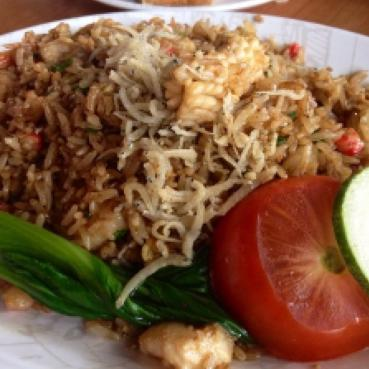
\includegraphics[width = \myfigurewidth\textwidth]{figures/vit-figures/8/fried_rice/original.jpg}}}$ &
    $\vcenter{\hbox{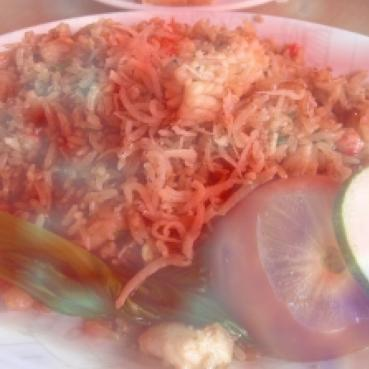
\includegraphics[width = \myfigurewidth\textwidth]{figures/vit-figures/8/pad_thai/standard_cam.jpg}}}$ &
    $\vcenter{\hbox{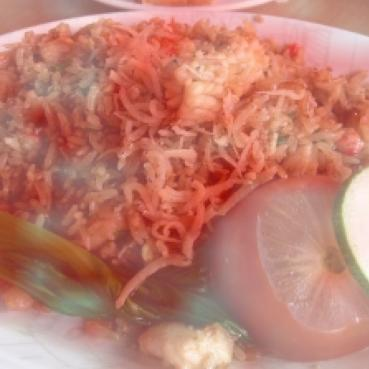
\includegraphics[width = \myfigurewidth\textwidth]{figures/vit-figures/8/pad_thai/standard_cam_w_relu.jpg}}}$ &
    $\vcenter{\hbox{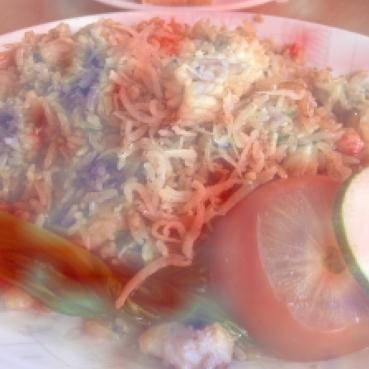
\includegraphics[width = \myfigurewidth\textwidth]{figures/vit-figures/8/pad_thai/contrastive_cam.jpg}}}$ \\

    \vspace{0.09cm}
    % \thead{Chocolate \\ Sauce} &
    $\vcenter{\hbox{\shortstack{\textbf{Fried rice} \\ p=0.45}}}$ &
    $\vcenter{\hbox{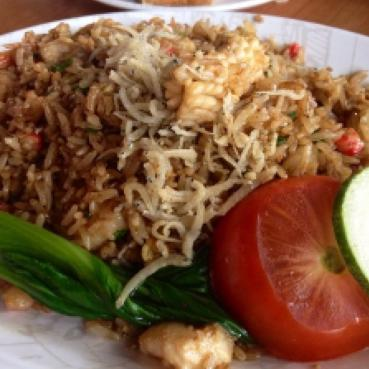
\includegraphics[width = \myfigurewidth\textwidth]{figures/vit-figures/8/fried_rice/original.jpg}}}$ &
    $\vcenter{\hbox{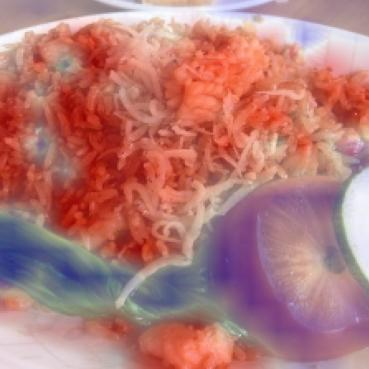
\includegraphics[width = \myfigurewidth\textwidth]{figures/vit-figures/8/fried_rice/standard_cam.jpg}}}$ &
    $\vcenter{\hbox{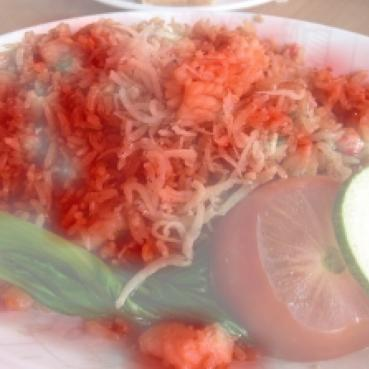
\includegraphics[width = \myfigurewidth\textwidth]{figures/vit-figures/8/fried_rice/standard_cam_w_relu.jpg}}}$ &
    $\vcenter{\hbox{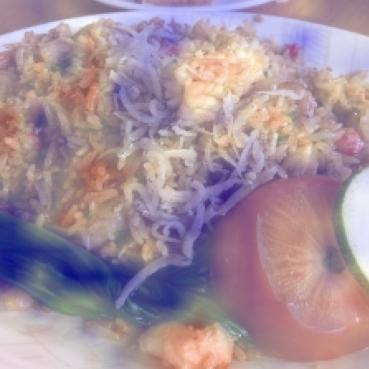
\includegraphics[width = \myfigurewidth\textwidth]{figures/vit-figures/8/fried_rice/contrastive_cam.jpg}}}$ \\


    \vspace{0.09cm}
    % $\vcenter{\hbox{Digital Watch}}$ &
    % \thead{Digital \\ Watch} &
    $\vcenter{\hbox{\shortstack{\textbf{Sushi} \\ p=0.35}}}$ &
    $\vcenter{\hbox{\includegraphics[width = \myfigurewidth\textwidth]{figures/vit-figures/10/sushi/original.jpg}}}$ &
    $\vcenter{\hbox{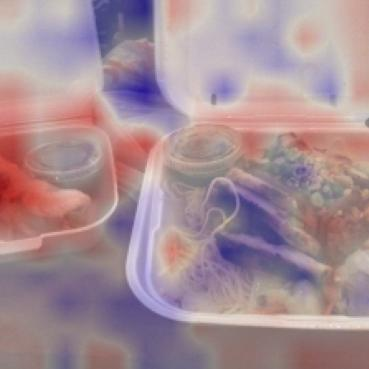
\includegraphics[width = \myfigurewidth\textwidth]{figures/vit-figures/10/sushi/standard_cam.jpg}}}$ &
    $\vcenter{\hbox{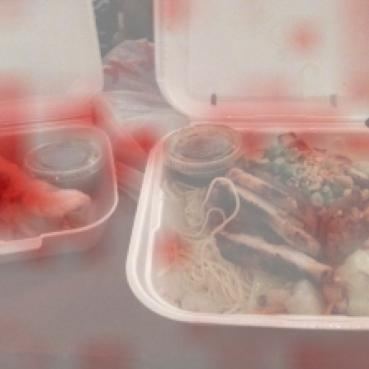
\includegraphics[width = \myfigurewidth\textwidth]{figures/vit-figures/10/sushi/standard_cam_w_relu.jpg}}}$ &
    $\vcenter{\hbox{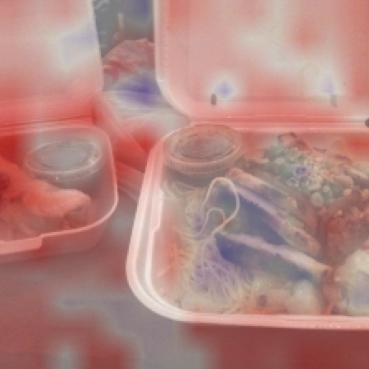
\includegraphics[width = \myfigurewidth\textwidth]{figures/vit-figures/10/sushi/contrastive_cam.jpg}}}$ \\

    \vspace{0.09cm}
    % $\vcenter{\hbox{Stopwatch}}$ &
    % \thead{Stop-\\watch} &
    $\vcenter{\hbox{\shortstack{\textbf{Ramen} \\ p=0.13}}}$ &
    $\vcenter{\hbox{\includegraphics[width = \myfigurewidth\textwidth]{figures/vit-figures/10/ramen/original.jpg}}}$ &
    $\vcenter{\hbox{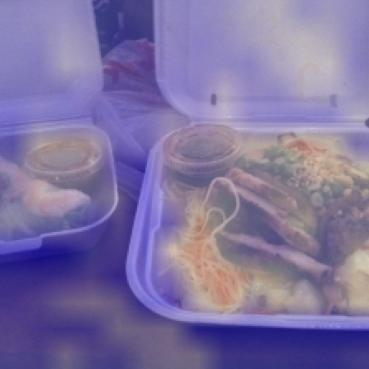
\includegraphics[width = \myfigurewidth\textwidth]{figures/vit-figures/10/ramen/standard_cam.jpg}}}$ &
    $\vcenter{\hbox{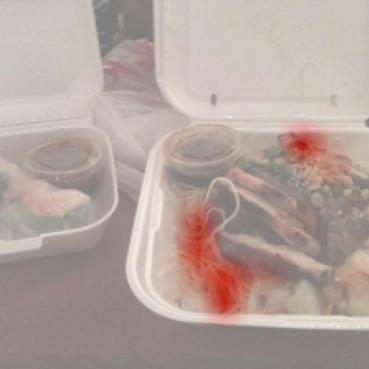
\includegraphics[width = \myfigurewidth\textwidth]{figures/vit-figures/10/ramen/standard_cam_w_relu.jpg}}}$ &
    $\vcenter{\hbox{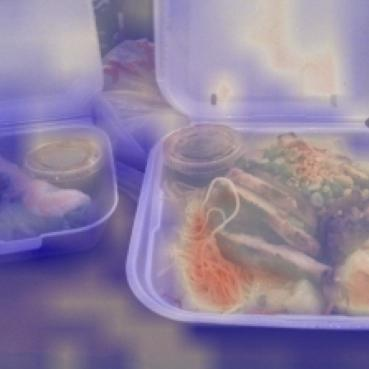
\includegraphics[width = \myfigurewidth\textwidth]{figures/vit-figures/10/ramen/contrastive_cam.jpg}}}$ \\

\end{tabular}
\caption{} \label{t:}
\label{fig:vit-gradcam-new-a}
\end{subfigure}

\begin{subfigure}{.5\textwidth}
\begin{tabular}
{ 
c@{\hspace{0.09cm}} c@{\hspace{0.09cm}} c@{\hspace{0.09cm}} c@{\hspace{0.09cm}} c@{\hspace{0.09cm}}}
    & \thead{Original} & \thead{GWAR} & \thead{GWAR \\ w/o ReLU} & \thead{Contrastive \\ GWAR} \\
    
    \vspace{0.09cm}
    $\vcenter{\hbox{\shortstack{\textbf{Pad thai} \\ p=0.53}}}$ &
    $\vcenter{\hbox{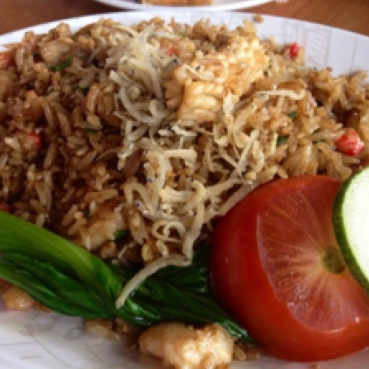
\includegraphics[width = \myfigurewidth\textwidth]{figures/vit-figures/results/2735232original_70.png}}}$ &
    $\vcenter{\hbox{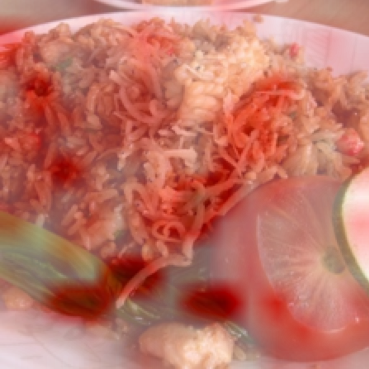
\includegraphics[width = \myfigurewidth\textwidth]{figures/vit-figures/results/2735232standard_70.png}}}$ &
    $\vcenter{\hbox{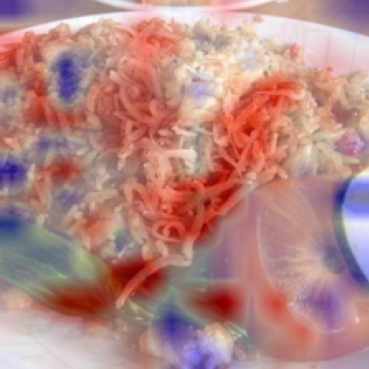
\includegraphics[width = \myfigurewidth\textwidth]{figures/vit-figures/results/2735232standard_contrastive_70.png}}}$ &
    $\vcenter{\hbox{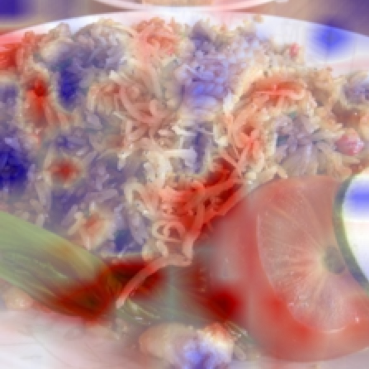
\includegraphics[width = \myfigurewidth\textwidth]{figures/vit-figures/results/2735232contrastive_70.png}}}$ \\

    \vspace{0.09cm}
    $\vcenter{\hbox{\shortstack{\textbf{Fried rice} \\ p=0.45}}}$ &
    $\vcenter{\hbox{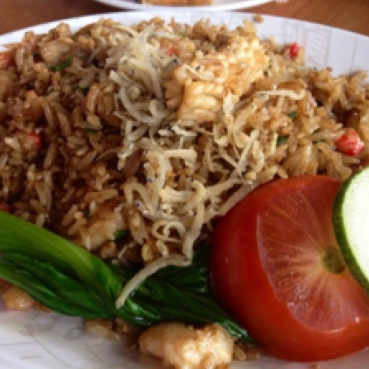
\includegraphics[width = \myfigurewidth\textwidth]{figures/vit-figures/results/2735232original_44.png}}}$ &
    $\vcenter{\hbox{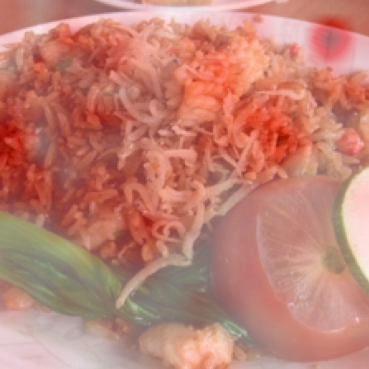
\includegraphics[width = \myfigurewidth\textwidth]{figures/vit-figures/results/2735232standard_44.png}}}$ &
    $\vcenter{\hbox{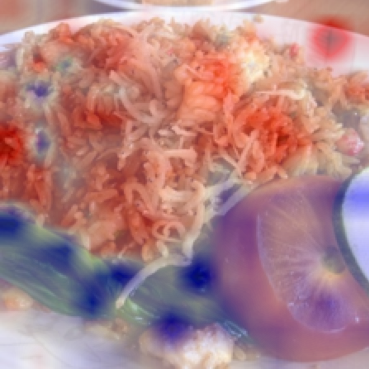
\includegraphics[width = \myfigurewidth\textwidth]{figures/vit-figures/results/2735232standard_contrastive_44.png}}}$ &
    $\vcenter{\hbox{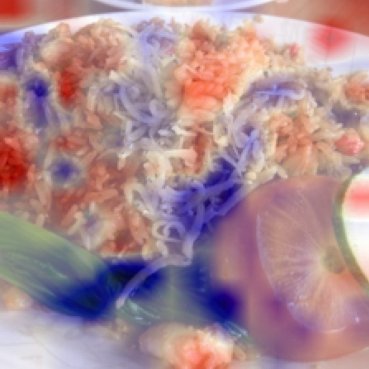
\includegraphics[width = \myfigurewidth\textwidth]{figures/vit-figures/results/2735232contrastive_44.png}}}$ \\

    \vspace{0.09cm}
    $\vcenter{\hbox{\shortstack{\textbf{Sushi} \\ p=0.35}}}$ &
    $\vcenter{\hbox{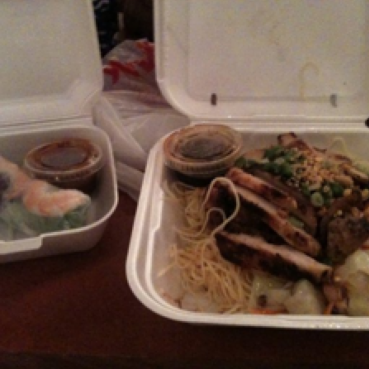
\includegraphics[width = \myfigurewidth\textwidth]{figures/vit-figures/results/945742original_95.png}}}$ &
    $\vcenter{\hbox{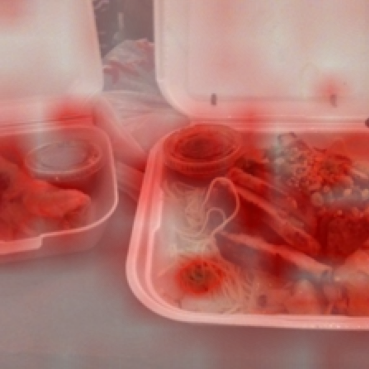
\includegraphics[width = \myfigurewidth\textwidth]{figures/vit-figures/results/945742standard_95.png}}}$ &
    $\vcenter{\hbox{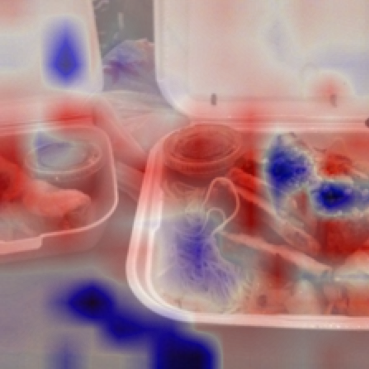
\includegraphics[width = \myfigurewidth\textwidth]{figures/vit-figures/results/945742standard_contrastive_95.png}}}$ &
    $\vcenter{\hbox{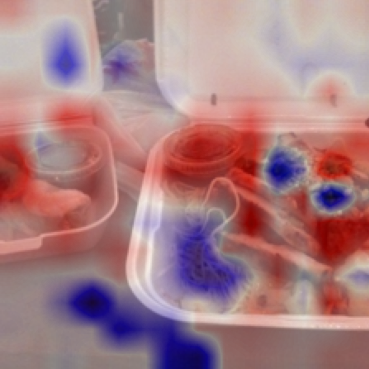
\includegraphics[width = \myfigurewidth\textwidth]{figures/vit-figures/results/945742contrastive_95.png}}}$ \\
    
    \vspace{0.09cm}
    $\vcenter{\hbox{\shortstack{\textbf{Ramen} \\ p=0.13}}}$ &
    $\vcenter{\hbox{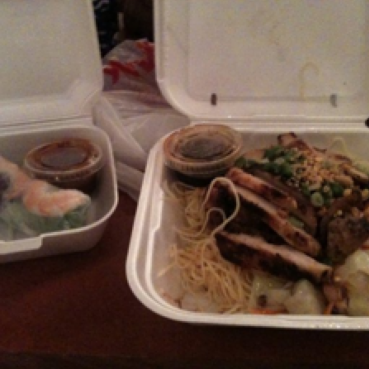
\includegraphics[width = \myfigurewidth\textwidth]{figures/vit-figures/results/945742original_81.png}}}$ &
    $\vcenter{\hbox{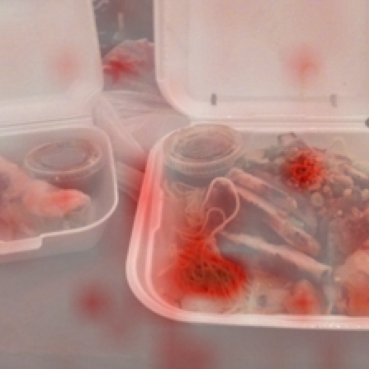
\includegraphics[width = \myfigurewidth\textwidth]{figures/vit-figures/results/945742standard_81.png}}}$ &
    $\vcenter{\hbox{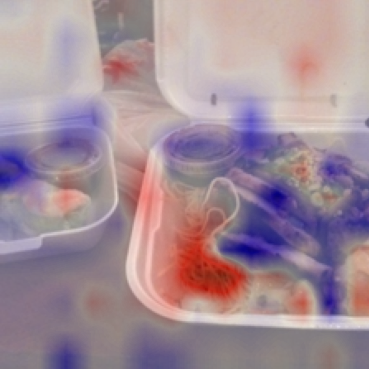
\includegraphics[width = \myfigurewidth\textwidth]{figures/vit-figures/results/945742standard_contrastive_81.png}}}$ &
    $\vcenter{\hbox{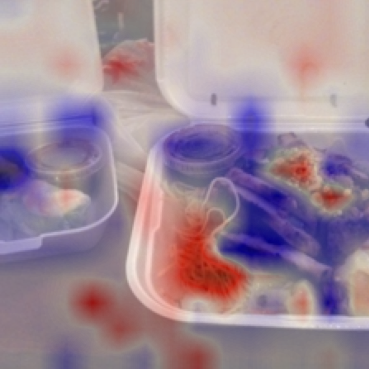
\includegraphics[width = \myfigurewidth\textwidth]{figures/vit-figures/results/945742contrastive_81.png}}}$ \\

\end{tabular}
\caption{} \label{fig:vit-gradcam-new-b}
\end{subfigure}
}

\caption{Comparison between proposed explanations. In (a) a comparison between GradCAM, GradCAM without ReLU, and Contrastive GradCAM is considered with target attention layer 8 and 10 respectively. In (b) a comparison between Gradient-weighted Attention rollout (GWAR) of the standard, without ReLU, and contrastive variant is considered. Red sections are considered areas with high explainability. To adapt the method to the contrastive version all ReLU operations were removed and the gradients were calculated from the softmax output instead of the logits.} \label{t:}
\end{figure}